\chapter{RELATED WORKS}
\label{Chapter 2}
\lhead{Chapter 2. \emph{Related Works}}

\section{Device Free Human Activity Recognition using WiFi Channel State Information}
In this study \cite{9060143}, the authors implemented an activity detection system using wifi channel state information. They were able to detect human activities like Walk, Stand, Sit, Run, etc. in a Line of Sight scenario (LOS) and a Non-Line of Sight (N-LOS) scenario within an indoor environment. They used two algorithms for classification, Support Vector Machine (SVM) and Long Short-Term Memory (LSTM) recurrent neural network. To collect the data, they used Intel WiFi Link 5300 Network Interface Card (NIC). This card supports the 802.11n standard and hence makes it possible to record channel state information. There are 64 subcarriers in 20 MHz channel and 128 subcarriers in 40 MHz channel. Two Lenovo laptops were used which were equipped with Intel WiFi Link 5300 Network Interface Card (NIC). The operating system on said laptops was 64 Bit Ubuntu version 14.04 LTS. The kernel version was 4.2.0-42. They modified the hardware using instructions provided by  Halperin et al. \cite{10.1145/1925861.1925870} who proposed the ‘Linux 802.11n CSI Tool”. For classification with SVM, they performed preprocessing and feature extraction using Discrete Wavelet Transform (DWT), Principal Component Analysis (PCA), etc, and then used the classifier. For classification with LSTM, only CSI-extraction and denoising were done. They achieved results where precision, recall, and F1 score were 95, 98, and 96 respectively for their best model.
\begin{figure}[H]
\centering
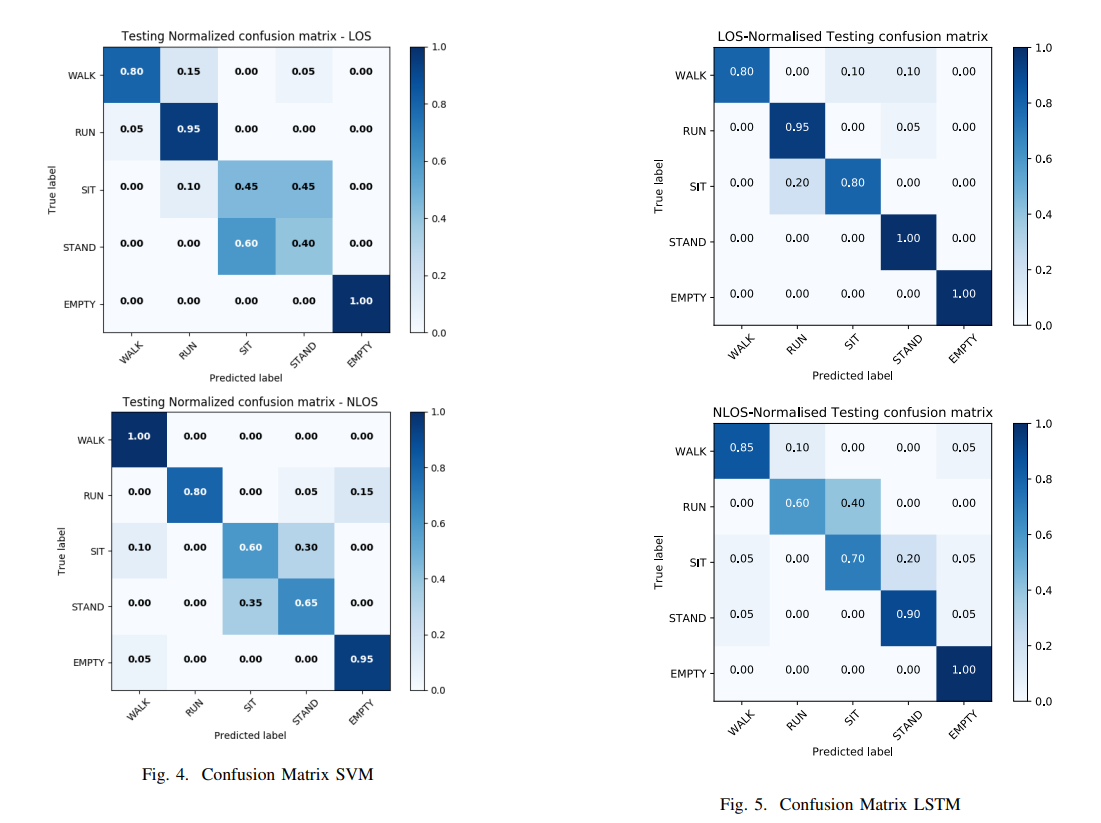
\includegraphics[width=1\textwidth]{./figure/chap 2/figure-1.png}
\caption{Confusion matrices in the paper}
\label{2.1}
\end{figure}

\textbf{There are some limitations in this method:}

\begin{itemize}
\item The hardware used for the experiment was two laptops, making this solution impractical for use in a real-world scenario. 
\item The system shows lower accuracy in detecting activities involving slow movement, like sitting or walking.
\item The system does not generalize for different environments.
\end{itemize}



\section{Wi-Motion: A Robust Human Activity Recognition Using WiFi Signals}
This study \cite{8873550}proposes a wifi-based human activity recognition system, Wi-Motion. The authors were able to classify five different pre-defined activities with impressive accuracy. The system showed a 96\% accuracy in line of sight arrangement and 92\% accuracy in non-line of sight arrangement. Furthermore, the authors evaluate the effect of the age of the experimental subjects and relatively complex environments. Wi-Motion jointly leverages the amplitude and phase information extracted from the CSI sequence. The authors first construct the classifiers using amplitude and phase, respectively. The output of classifiers is then combined by a posterior probability-based combination strategy. The authors used a commercial Tp-Link wireless router as the transmitter operating in the IEEE 802.11n AP mode at 2.4GHz. An Acer Aspire EC laptop running Ubuntu 14.04 was used as a receiver, which is equipped with an off-the-shelf Intel 5300 card (three antennas) and a modified firmware. During the process of receiving WiFi signals, the receiver pings the router 33 pkts/s and records the CSI of each packet. For each activity in different environments, every user provides 30 instances to evaluate the performance of their system. Two complex office environments were selected for data collection and 6 participants provided the data. They extracted amplitude features using DWT (Discrete Wavelet Transform). The phase feature extraction is done using WMA method and PCA. The authors use a support vector machine (SVM) algorithm for the classification of the five activities:
\begin{enumerate}
    \item Bend
    \item Halve squat
    \item Step
    \item Stretch leg
    \item Jump
\end{enumerate}

The authors also showed that the system provided accuracy higher than 80\% even when there were multiple users present. Moreover, they showed with their analysis that  during the process of data collection,
the physiological function of the person decays as the age increases, which makes the movement slower and difficult to control in a stable situation.

\begin{figure}[H]
\centering
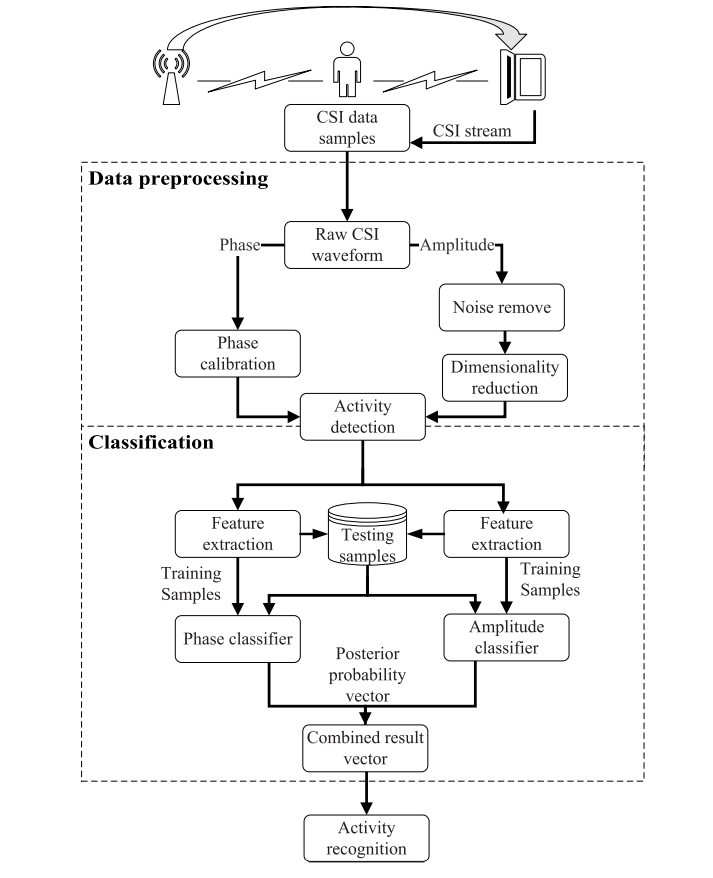
\includegraphics[width=1.0\textwidth]{./figure/chap 2/2.png}
\caption{System structure for Wi-Motion}
\label{2.2}
\end{figure}


\begin{figure}[H]
\centering
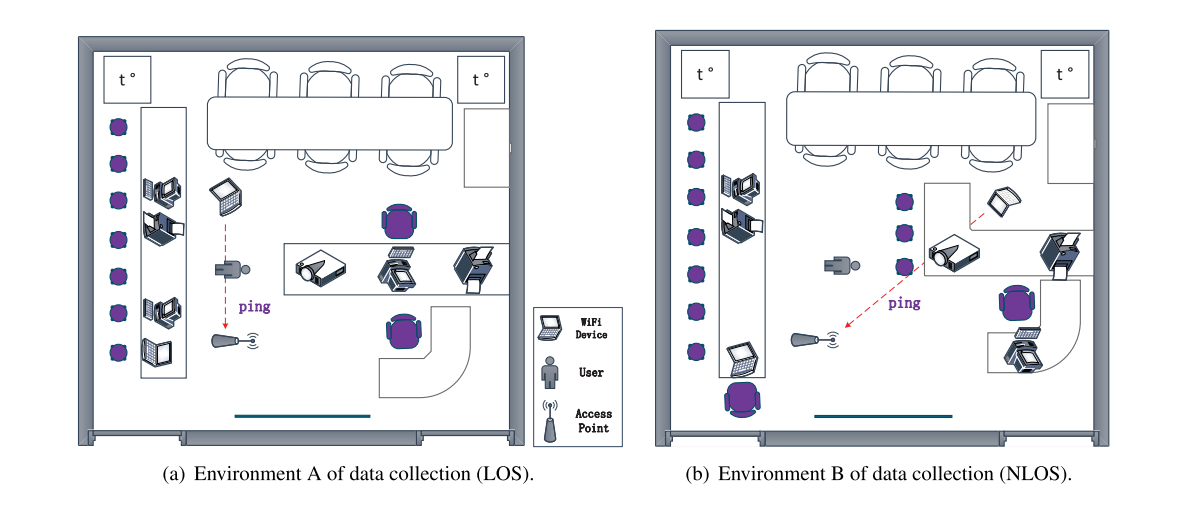
\includegraphics[width=1.0\textwidth]{./figure/chap 2/3.png}
\caption{Environment set of data collection.}
\label{2.3}
\end{figure}
 
 \textbf{Limitations:}

\begin{itemize}
\item The hardware used for the experiment were two laptops, making this solution impractical for use in a real-world scenerio. 
\end{itemize}

\section{MultiSense: Enabling Multi-person Respiration Sensing with Commodity WiFi}
The study \cite{10.1145/3411816} proposes Multisense, a WiFi-based system that can continuously
sense the detailed respiration patterns of multiple persons. It can provide a robust performance even if they have very similar respiration rates and are physically closely located. The main contributions of the paper are as follows:
\begin{itemize}
    \item The authors offered a novel method for canceling out the time-varying phase offset of WiFi CSI without distorting the linear mixture. 
    \item They showed that respiration sensing can be treated as a BSS problem that the ICA approach can efficiently address.
    \item They put MultiSense on common WiFi devices and ran comprehensive tests to see how well it works.
\end{itemize}

The authors collected CSI data using the CSI tool \cite{7010501}, which reports the complex-valued CSI samples for each received packet and can be used to collect CSI data from the receiver. For reporting CSI, the Intel 5300 WiFi card in the receiver is set to run at 5.24 GHz with a sample rate of 200 Hz and provides CSI information on 30 sub-carriers. The transmitter and receiver are both equipped with three antennas unless otherwise noted.

\begin{figure}[H]
\centering
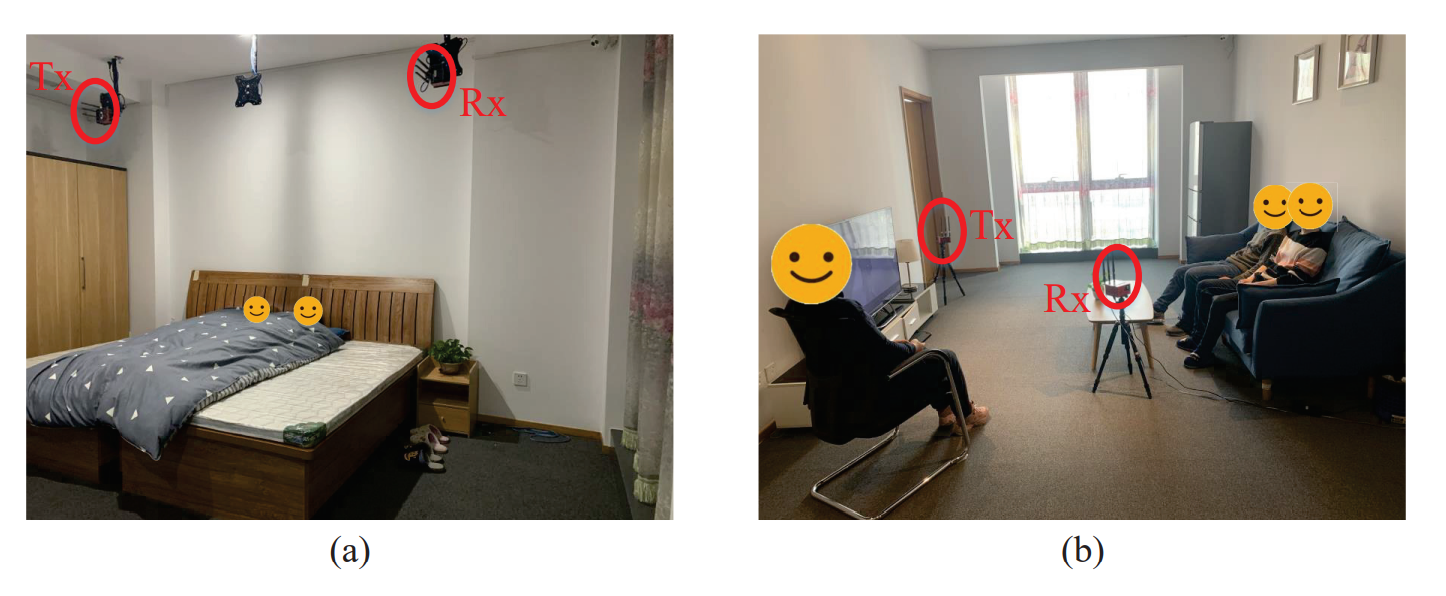
\includegraphics[width=1.0\textwidth]{./figure/chap 2/4.png}
\caption{The experimental setup in two scenarios: (a) all subjects sleep on a bed in the bedroom;
(b) each subject sits on a couch or chair in the living room.}
\label{2.4}
\end{figure}

The authors used ICA (Independent Component Analysis) to separate the breathing patterns of different persons. The added time-varying phase offset (t) and background static signals affect CSI from commodity WiFi. As a result, using raw CSI retrieved from commodity WiFi equipment, the authors were unable to use ICA to distinguish multi-person respiration signals. To overcome this, they proposed a novel method where they canceled the time-variant phase offset and removed the background static signal. Even in the presence of four people and only a pair of Wi-Fi transceivers, MultiSense is quite accurate, with a mean absolute respiration rate inaccuracy of 0.73 bpm.

\begin{figure}[H]
\centering
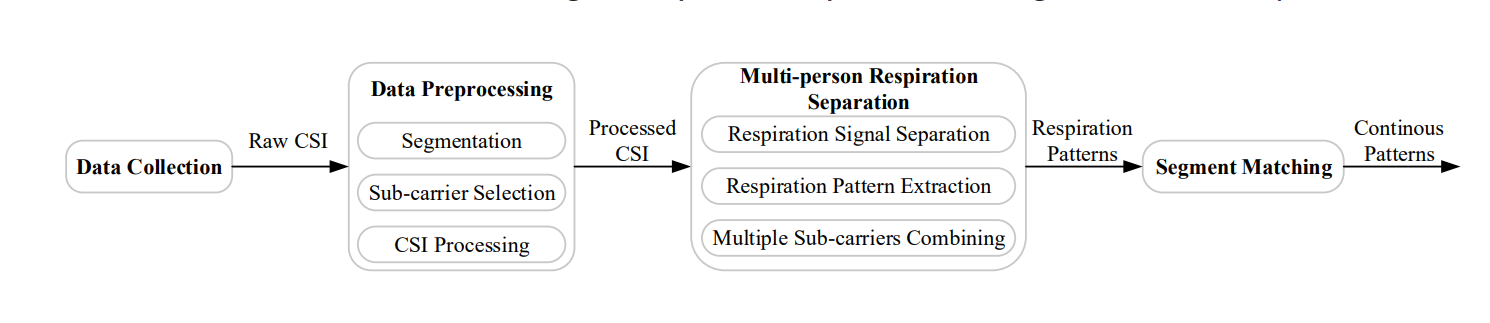
\includegraphics[width=1.0\textwidth]{./figure/chap 2/5.png}
\caption{The MultiSense system overview.}
\label{2.5}
\end{figure}

 \textbf{Limitations:}

\begin{itemize}
\item When performing blind source separation using ICA method, the number of persons is required as the input as an inherent characteristic of ICA is that it cannot identify the actual number of source signals in general. 
\item The system is not able to assign the breathing patterns to users in the case of multiple persons.
\end{itemize}

\section{A Wireless-Vision Dataset for Privacy Preserving Human Activity Recognition}
This study \cite{9264288} proposes a new WiFi-based and video-based neural network (WiNN) to improve the robustness of activity recognition where the synchronized video serves as the supplement for the wireless data. In three different visual circumstances, including scenes without occlusion, partial occlusion, and full occlusion, a wireless-vision benchmark (WiVi) is gathered for 9 class actions recognition. The accuracy of the data set is verified using both machine learning methods - support vector machine (SVM) and deep learning methods. The authors show that the WiVi data set meets the primary demand and that all three branches of the proposed pipeline maintain accuracy of more than 80\% for multiple action segmentation from 1s to 3s. 

\begin{figure}[H]
\centering
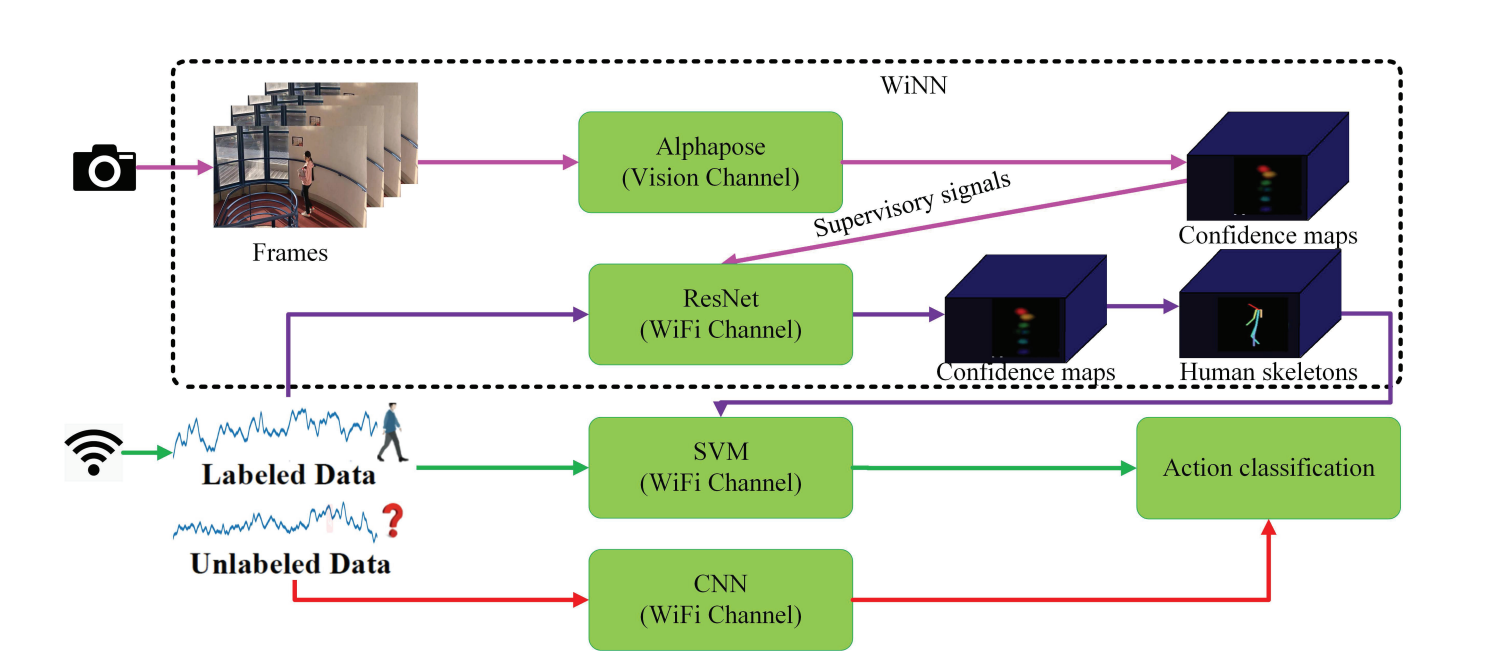
\includegraphics[width=1\textwidth]{./figure/chap 2/6.png}
\caption{The flowchart of the network for WiVi dataset.}
\label{Fig 2.6}
\end{figure}

The contribution of the paper can be summarized by the following points:

\begin{itemize}
    \item To test the effectiveness of existing activity identification systems, the authors first created WiVi, a wireless-vision activity data set. To verify the WiVi dataset's effectiveness, they used SVM, Convolutional Neural Networks (CNN), and WiNN.
    \item The authors proposed the WiNN, a WiFi-based and video-based neural network for activity recognition in partial and full occlusion scenarios, which improves the robustness of activity recognition using synchronous video as a supplement and complement to WiFi CSI signals.
    \item To verify the quality of the WiVi data set, the authors compared the machine learning method SVM with the deep learning methods CNN and WiNN. WiNN, in particular, delivered the most reliable results for multiple action segmentation from 1 to 3 seconds.
\end{itemize}

\begin{figure}[H]
\centering
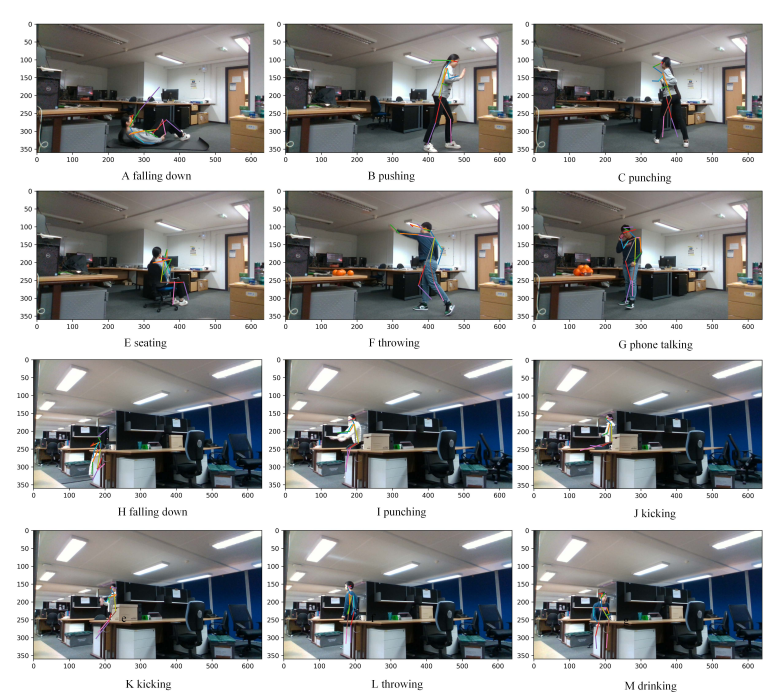
\includegraphics[width=1\textwidth]{./figure/chap 2/7.png}
\caption{The visual skeleton result of the CSI in two scenarios, where A-G are without occlusion scene, and H-M are partial occlusion scene.}
\label{Fig 2.7}
\end{figure}

 \textbf{Limitations:}

\begin{itemize}
\item The number of participants was very small. 
\item The baseline SVM model performed better than their proposed WiNN model.
\end{itemize}